
\section{The IMF Ecosystem}
\label{ch:Chapter 7}

- icons
- best practices, recommendations
- end-to-end example?

In order to describe a typical set up of an IMF Ecosystem, we use the
following terminology:

\begin{description}
\item[{IT Ecosystem}] IT ecosystem refers to an orchestrated
  collection of components: IT systems, tools, actors and roles, and
  how they interact to achieve a specific goal.

\item[{Data}] Data refers to the information that is stored,
  processed, and transmitted within the IT ecosystem. It can include
  text, numbers, images, audio, video, or any other form of digital
  content.

\item[{Language and Format}] Language and format refer to the methods
  and standards used for communication and data representation within
  the IT ecosystem. This includes data exchange protocols and data
  formats that dictate how data is structured and transmitted.

\item[{IT Systems}] IT systems are the major components within the IT
  ecosystem that store data and provide services that process data.
  Typical examples are databases and server-side applications.

\item[{Tools}] Tools refer to software applications, utilities, or
  programs that are used to perform specific tasks or functions,
  typically on data, within an IT ecosystem. They can be used for data
  analysis, editing, monitoring, or other purposes. Typical examples
  are client side desktop applications.

\item[{Service}] A service is a specific functionality or capability
  offered by an IT system or tool. It defines what the IT system or
  tool can do and how it can be accessed or utilized by
  actors. Typical examples of services are data validation, identifier
  management, and user authentication.

\item[{Actors}] Actors represent entities or users that interact with
  IT systems and tools. They can be individuals, external systems, or
  automated processes that initiate actions or provide input to the
  system.

\item[{Roles}] Roles represent the different functions or
  responsibilities that individuals or components within a IT
  ecosystem have. They define who or what performs specific tasks or
  operations within the system.
\end{description}

\subsection{IMF Ecosystem Components}

\subsubsection{Reference Data}
\label{sec:reference-data}

Reference data refers to a specific type of data that provides context
or categorization for other data. It is typically static and does not
change frequently, serving as a point of reference or standard against
which other data can be compared, classified and integrated. Reference
data is used for validation, to ensure consistency and complience,
accuracy, to organise data within an IT ecosystem, and to standardise
access and use of data in the IT ecosystem.

In the IMF ecosystem, reference data appear in the form of reference
data items (classes, relations and individuals) typically defined in
international domain standards, such as ??? IDO, eCLass, ...? that
define industry shared resources such as equipment classes and units of
measure.

We also refer to standardised graphical symbols used for diagrams,
such as P\&ID diagrams, as reference data.

Reference data is typically made accessible by reference data
libraries.


\subsubsection{Reference Data Library}
\label{sec:refer-data-libr}

A reference data library (RDL) is an IT system whose main service is
to publish reference data so that it can be referred to by other systems, tools and
data. 
Additionally, an RDL may provide services like
data validation,
data analysis,
data enrichment,
data governance,
and
creation and curation of reference data.
These services are typically offered through APIs and are used via purpose built tools.

The IMF ecosystem contains different kinds of reference data
libraries:
industry terminology RDLs that contain industry shared terms such as equipment classes and units of measure; 
symbol RDLs that contain standardised graphical symbols;
and
IMF type libraries.

\subsubsection{IMF Type Library}

An IMF type library is a reference data library that publishes IMF types.

The benefits of an IMF type library, in addition to the generic benefits of reference data libraries, is to reduce the startup costs of using IMF as an IMF type library will provide useful IMF modelling patterns for use in the creation of IMF models.

In addition, an IMF type library may provide the following services:

\begin{itemize}
\item Submitting suggestions for new and updating existing IMF types.
\item Quality assurance (QA) process for approval of suggestions for
  new and updating existing IMF types. The QA workflow shall be
  transparent and offer relevant tools for an efficient and easy to
  use workflow.
\item Versioning scheme for the entries in the library.
\item APIs that allow for querying the library.
\item Classification schema for the IMF types.
\end{itemize}
  
An IMF type library should be community driven and allow users to submit new IMF types and update already
existing IMF types in the library. This will allow users across the industry and value chain to collaborate to create
high quality content. The approval process can be implemented as a peer-review where groups of SMEs can collaborate
to ensure that updates to the library have the necessary quality.

The API of the IMF type library shall offer support for required functionality in
the IMF type editor tools and IMF modelling tools.


\paragraph{Symbol Library}
\label{sec:symbol-library}

\paragraph{Data Hub}


\paragraph{Source databases}


\subsubsection{Tools}
\label{sec:tools}

\subsubsection{IMF Type Editor Tool}
An IMF type editor is used to create new IMF types, modify existing IMF types, and publish IMF types in a IMF type library.

An IMF type editor tool shall offer support for:

\begin{itemize}
  \item Search and browse for existing IMF types in IMF type libraries.
  \item Interaction with reference data library for finding and referencing reference data items such as attributes, classes.
  \item Creation of new IMF types using user interfaces adapted to SMEs.
  \item Updating existing IMF types in an IMF type library.
  \item A workflow for submitting new or updating existing IMF types in an IMF type library.
  \item A workflow for submitting suggestions for new reference data entries to a reference data library.
\end{itemize}
To increase the standardisation of the types created using an IMF type editor tool, reference data libraries
previously described shall be used for sourcing attributes, symbols, and classes for the creation of IMF types. There
should be a workflow that allows the SME to submit suggestions for new reference data entries to an RDL that are
identified as missing during the IMF type creation process.

An IMF modelling tool is used by SMEs to create and share IMF models.

An IMF modelling tool shall offer support for:

\begin{itemize}
\item A graphical user interface adapted to SMEs.
\item Searching and browsing for types in IMF type libraries.
\item Creation of IMF models using the complete spectrum of the IMF language.
\item Export and import IMF models to and from the IMF language.
\item Enabling plugins, e.g., that perform specific calculations and queries.
\end{itemize}
IMF modelling tools shall source the IMF types from an IMF type library. The sourced IMF types are then instantiated
in the modelling tool. Setting the values or references to values for the different attributes of the IMF types shall
be possible in the modelling tool.

An IMF modelling tool should provide a framework for adding plugins to, e.g., perform calculations and queries on the created
model.

\subsubsection{Languages and Formats}
\label{sec:languages-formats}


The IMF Ecosystem is intended to be an industry wide collaboration that allows transfer
of Information Models between the different parts of the value chain (operators, engineering contractors, suppliers).
To enable seamless transfer of information models between the different actors, potentially using different
applications, a standardised serialisation and data exchange format is needed.

The formal specification of the IMF language, which is also used as a serialisation and exchange format, is found in \autoref{ch:The IMF Language Formalized}.
The data exchange format is defined using widely accepted W3C standards. The IMF data exchange format is Resource
Description Framework (RDF), using any of its widely supported standardised serialisation formats. Several
serialisation formats for RDF exist, including JSON-LD, which is based on JSON, and RDF/XML, which is based on XML.
The data exchange format vocabulary is specified using the Web Ontology Language (OWL) and its grammar is
defined using the Shapes Constraint Language (SHACL).


\subsection{Scenarios}
\label{sec:scenarios}



\subsection{Implementations}
\label{sec:implementations}

\paragraph{Open-Source tool \emph{:Tyle}.}

The IMF type editor \emph{:Tyle} has been developed to offer adopters of IMF a web-based open-source IMF type
editor. :Tyle supports creation of IMF types using reference data from the PCA RDL.
:Tyle is developed as an open source project, where all users are
invited to contribute to the development of the tool by submitting code, bug reports or feature requests. Source
code, documentation and user tutorials can be found on
\href{https://github.com/mimir-org/typelibrary}{Github}.



\paragraph{Open-Source Tool \emph{Mímir}.}

The open-source IMF modelling tool \emph{Mímir} has been developed to offer adopters of IMF a web-based open-source
modelling tool. It supports creation of models, sourcing types from an IMF type library and compiling the models into
ontologies. All users are welcome to contribute to the development of \emph{Mímir} by submitting code, bug reports
or feature requests. Source code, documentation and tutorials can be found on
\href{https://github.com/mimir-org/mimir}{Github}.


\subsection{OLD below}

\begin{figure}[htb]
  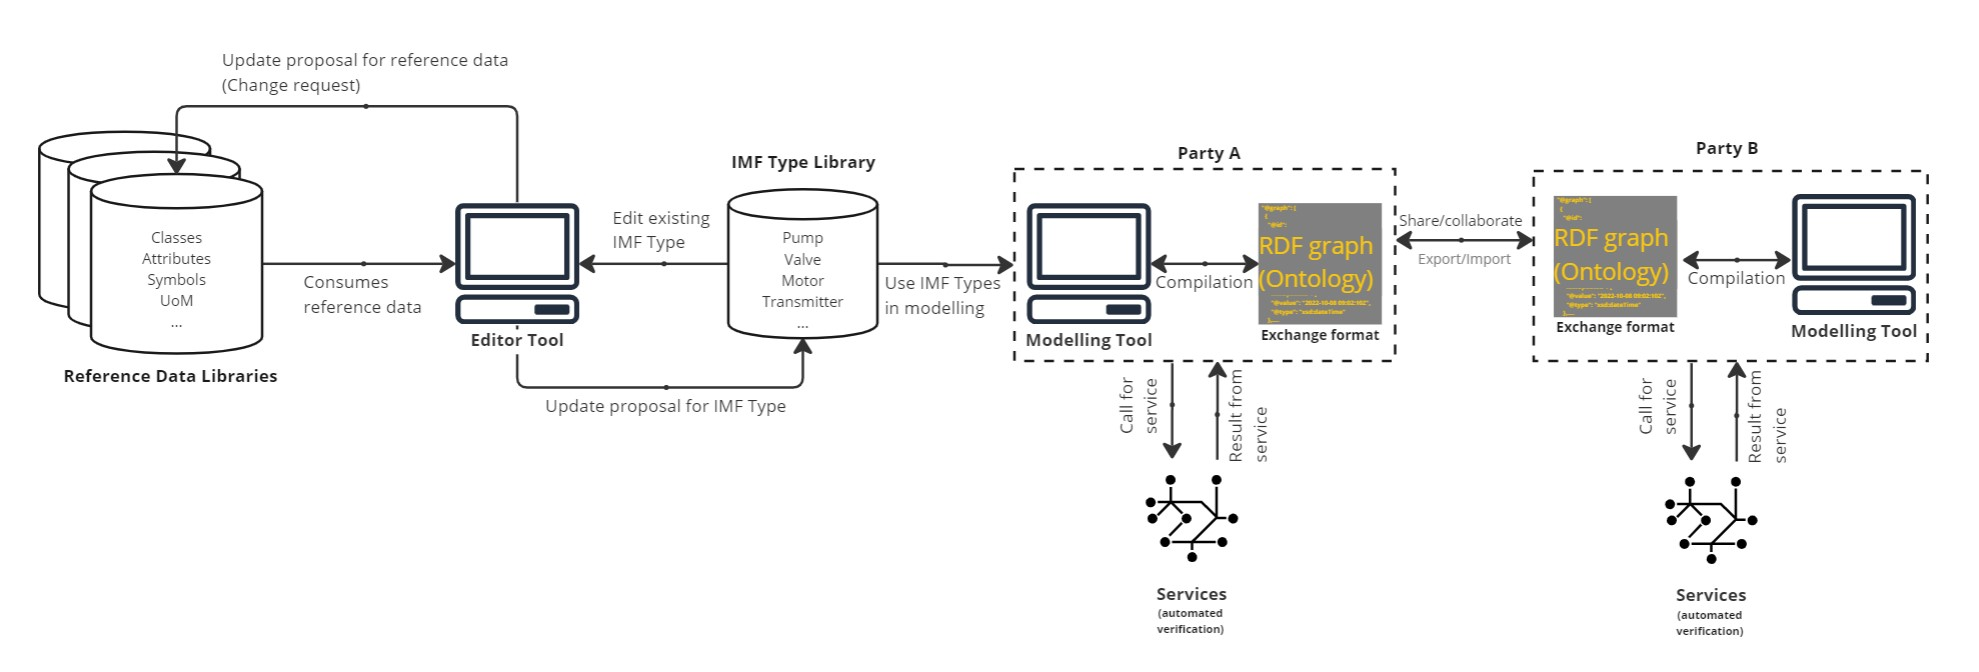
\includegraphics[width=1\textwidth]{img/IMFmanual-img072.jpg}
  \caption{Overview of the IMF ecosystem.}
  \label{fig:Figure 54}
\end{figure}


IMF will be implemented in the context of applications that serve
different parts of an ecosystem. The applications in the ecosystem should enable the engineers to create and
share information models with minimal training and independent of companies and industries. An overview of the
different components in the ecosystem is depicted in \autoref{fig:Figure 54}. The main components are reference data libraries, an IMF type library,
authoring tools, and data exchange formats. In this section all references to applications in the IMF ecosystem are
made to the type of application, not to a specific instance of the applications unless otherwise stated.


\subsection{Authoring Tools}

Authoring tools are front-end tools used by the SMEs to create IMF types and IMF
models. These tools can be implemented as standalone products or be integrated into already existing engineering
tools. 
%To offer seamless integration with the other components in the IMF ecosystem the implementation of the
Authoring tools must comply with the formal specification of the the IMF language (\autoref{ch:The IMF Language Formalized}).




%%% Local Variables:
%%% mode: latex
%%% TeX-master: "../wip"
%%% End:
